\chapter{Analysis and Development}
\section{Analysis}
\vspace{-0.5cm}
\subsection{Current System Analysis}
\label{subsec:CurrentSystemAnalysis}
%% bahas  tentang kondisi real yang dihadapi, tambahkan alur layanan saat ini, proses-proses evakuasi(done),
%% sama layanan bisnis yang tersedia(done).
To build a good service, it is necessary how the plan before, develop and manage of infrastructure development, products and services from Disaster Management. Planning, development and managing every processes and steps in reducing impact of disaster will reduce the victims directly.\par 
Indonesia Disaster Ecosystem is consist of 3 (three) main actors. They are the Government, Disaster Stakeholders and people (community). The government consist of local or national government that taking a part in disaster reduction. Stakeholders such as Indonesian Red Cross, Hospitals and disaster rescue team, and of course the communities are the main actors. As same as another country, Indonesian government has their disaster management model as shown in figure \ref{fig:idm_figure}. Recent condition, system is divided to three stages. Activity, phase and function. Each stage has important point.\par 
\begin{figure}[H]
\begin{center}
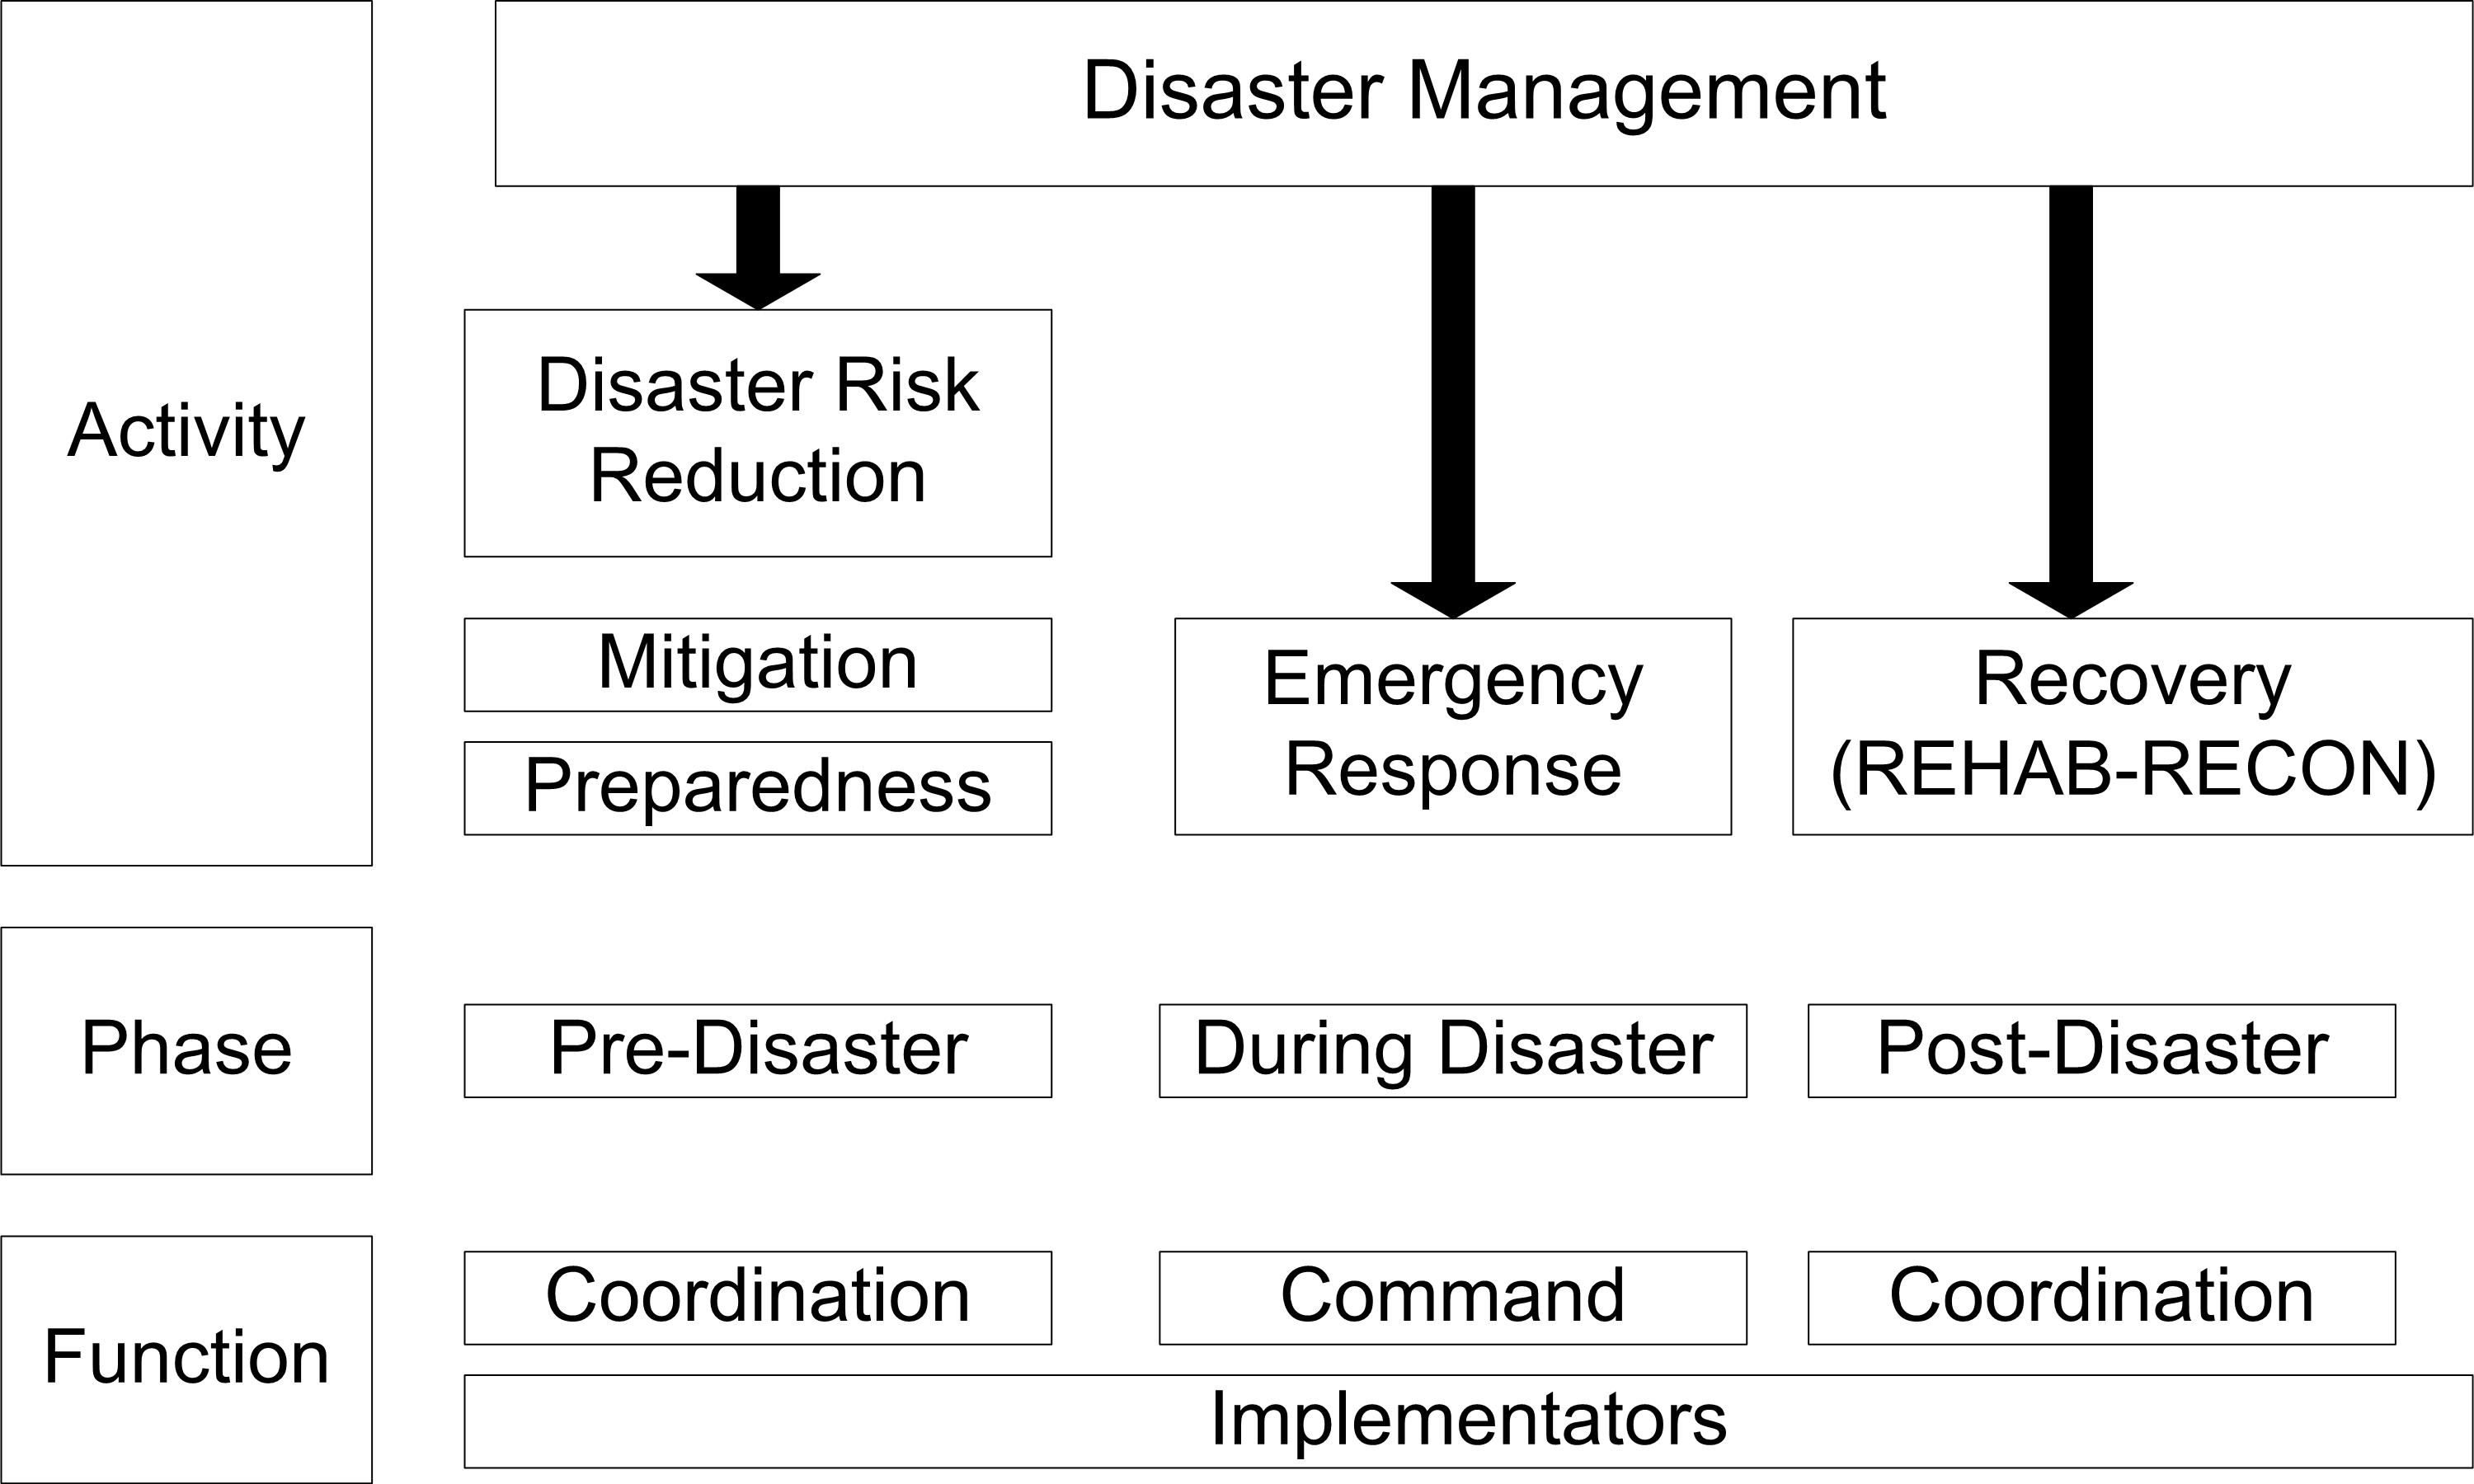
\includegraphics[scale=0.85]{idm.jpg}
\caption{Indonesian Disaster Management Today \cite{Framework2013}}
\label{fig:idm_figure}
\end{center}
\end{figure}

Disasters, both natural and man-made, can strike anytime or anywhere. There are two ways to overcome disasters: the first is preventing them from occurring, and second is having an emergency system and plan of operation prior to the occurrence of any crisis. In either approach, information technology plays an important role in crisis management. Disasters, like earthquakes, floods, etc. can cause large number of deaths, injuries and homeless people. Appropriate responses are needed in the form of allocating resources to handle the effects of disasters\par

In statement of problems, this research mentioned about the lack of DM-Regulation and Non-Regulation such as those related to investment and economic development. Disharmony in regulatory framework for Disaster Risk Reduction (DRR) also exists between different levels of government. Integration of DRR into sustainable development policies has been initiated through risk sensitive spatial planning and development plan, but they have not been widespread as people’s understanding of these issues is still limited.\par
Common perception of DRR and a common understanding of the way to mainstream DRR into development have also not been achieved. Many decision makers, including those at the executive and legislative branches of the government, still hold the opinion that disaster management is a matter of responding to disaster events, and therefore disaster policies and budget are more focused on disaster response and post-disaster recovery aspects. Another challenge is that the existing Disaster Risk Reduction (DRR) policies have not been implemented well and translated into capacity and institutional development. Many relevant policies have been formulated at the central level, but their implementation at the provinces and districts/cities have not been to the maximum. The existing government administration system still limits resources for disaster risk reduction.
Future\par 

\begin{figure}[H]
\begin{center}
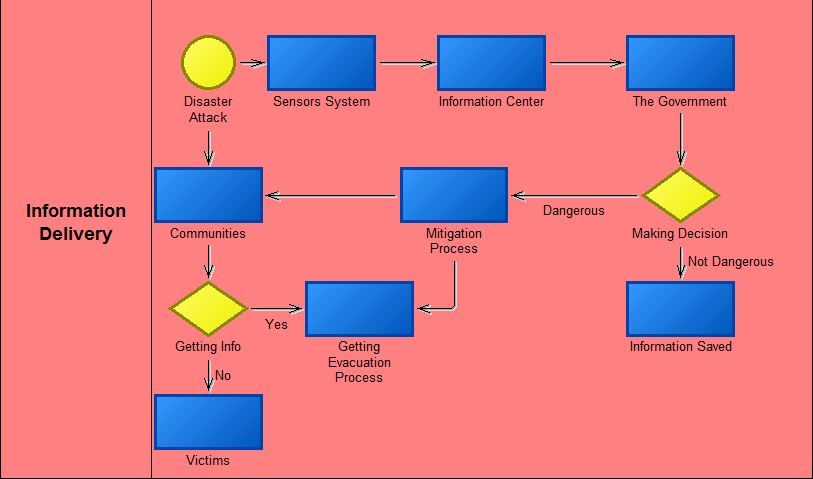
\includegraphics[scale=0.6]{BMbeforeSOA.png}
\caption{Information and Evacution Model Process}
\label{fig:EvaModel01}
\end{center}
\end{figure}

The figure \ref{fig:EvaModel01} above explain familiar process. The circulation mitigation process started after after disaster happen. The sensors that implemented to detect the disaster coming warn the communities, usually we call this with early warning. The information converted from sensor received by disaster information center. the next step is the decision making. The Government is a main actor here. Their decision need to be quick and precise, and the information will be delivered to communities. The process of delivering information  stopped here. Next step are depending on the communities, if they achieved the information and/or being in far from disaster location, they will be safe.\par
Figure \ref{fig:EvaModel01} also explained that current system not directly include disaster stakeholders.  Another stakeholders here can be Indonesian Red Cross (PMI), National Rescue Team Agency (BASARNAS) or Another National Disaster Mitigation Agency. Most of them got the information by themselves. Usually, The information comes from news media or from other people. Lack of information received effected to time of helping process. The rescue team came late to evacuation area and does not have enough preparation in area. The problem could be worse if the disaster attacked rural area.\par 

\begin{figure}[H]
\begin{center}
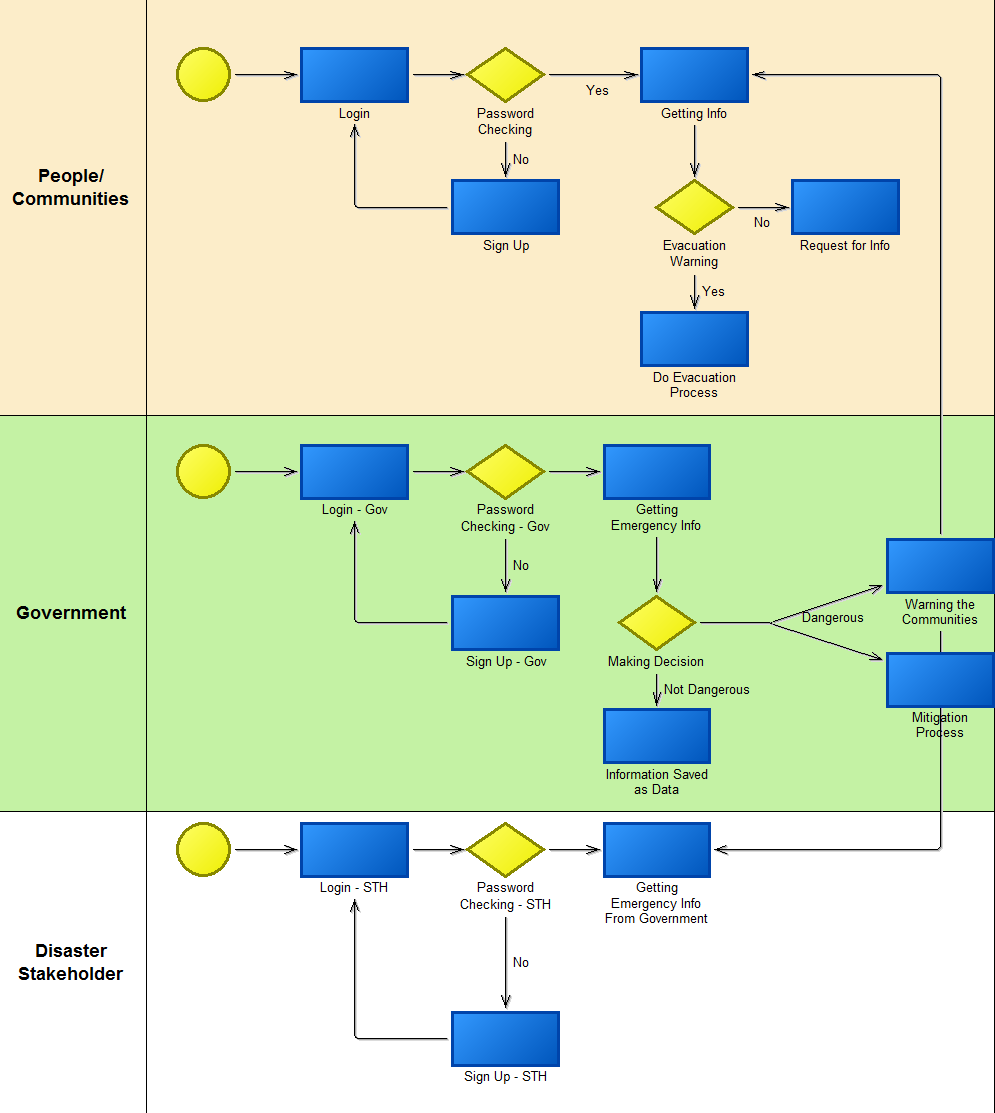
\includegraphics[scale=0.5]{BMafterSOA.png}
\caption{Business Process After Adding Services}
\label{fig:BisnisMOdelSOA}
\end{center}
\end{figure}
\par

As mentioned in  first section, this paper limit the research  in defining services needed and strategy to provide the DMS based on HFA. in the first section, many problems mentioned after implementation of HFA. Based on that cases, there are four main point government should do:\par

\begin{enumerate}
\setlength{\itemsep}{1.5pt}
\setlength{\parskip}{1.5pt}
\item Handling during disaster events that must be expedited.
\item Disaster education should be given to the society equally before the disaster occurred.
\item Handling of disasters should be evenly distributed in each region.
\item The coordination between government, stakeholders and many disaster management agency should be better addressed.
\end{enumerate}\par

Smart Disaster Management System (SDMS) also can be realized without four points above. Nevertheless, Indonesia is a country with large archipelago. Accordingly, SDMS in Indonesia can be created by modeling combination of various system with understanding of socio-economic states, technological advances and government policy. The growth of service science is going on to engineering sciences too. The service engineering can not be separated today. In many research we find that service engineering has been implemented in many sectors. Accordingly, we try to implement the service engineering method to disaster management system in Indonesia.\par

Business process designed (figure \ref{fig:BisnisMOdelSOA}) by adding some new element. The main actor in business process is government. Stakeholders added as the new element in business process. They will take a part in process of mitigation. The Government connected them directly to communities by sharing information as fast as they did to communities. By doing this, stakeholders/ disaster agency will come to disaster area soon after getting information with good preparation.\par

The information delivered to stakeholders in not only a part of small info about disaster happen. The information of location should be include in that short information. The location given is part of services. Using GPS technology at mobile phone and the disaster area informed, disaster rescue team can arrived at the area precisely.\par 

\section{SWOT Analysis}
Business Process Model is designed needs further analysis, therefore it takes a SWOT analysis. SWOT analysis is an analysis of internal and external conditions of an organization\ business process which in turn will be used as the basis for designing the strategy and working program. Internal analysis includes assessment of the strength factor (Strength) and weakness (Weakness), while the external analysis includes assessment of the chance factor (Opportunities) and challenges (Threats) of an organization / business process\cite{ThesisKangTeguh}.\par 
\begin{figure}[h]
\centering
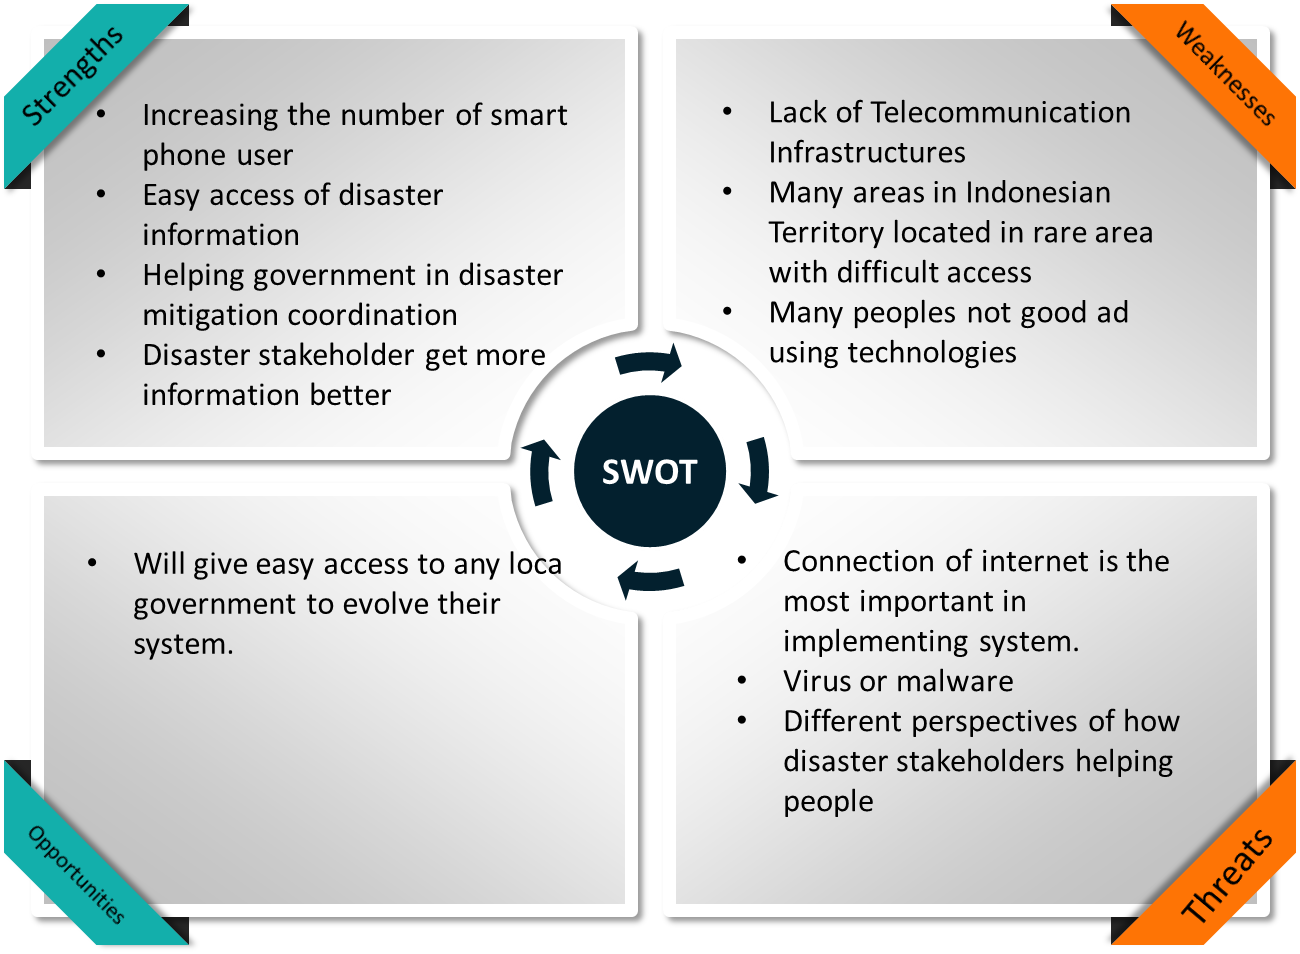
\includegraphics[scale=0.4]{SWOTAnalysis.png}
\caption{SWOT Analysis}
\label{fig:swot}
\end{figure}\par

%% sepertinya pada gambar analisa swot yang bagian opportunities perlu ditambahain opportunities untuk stakeholders dan disaster agency,,,, karena yang ada pun baru satu buah	

The strength and weakness, both are internal problems. The external problems are the opportunity and threats. From the figure \ref{fig:swot} we can define four main points from SWOT analysis. The strength of this system are lied at high amount of smart phone users, easy information accessed, and helping the government in giving disaster mitigation. The weakness comes from the dependency of system with internet connectivity. The dependency will be a problem in rural area of disaster location. In some condition, information can not be accessed. From internal analysis, the opportunity of system comes from easy access. The easy access of information by government will evolve their existing system. The last is the threats of the system. Main threats is from internet connection exactly. This problem mainly comes because of dependency with internet from system.\par 

\section{Service Oriented Analysis for Disaster Management}
Figure \ref{fig:SEFramework} explain 3 main step of designing the services. Thomas Erl (2006), detailed that 3 main steps to design a service, the detail steps mentioned in figure below:
\begin{figure}[H]
\centering
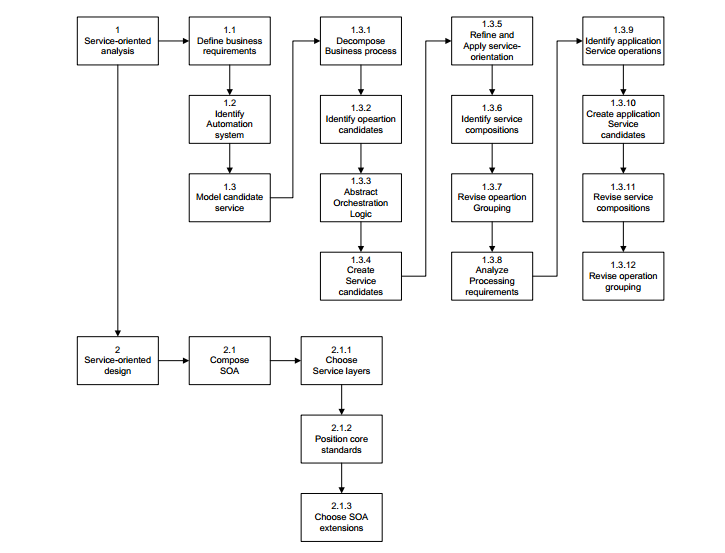
\includegraphics[scale=0.7]{desainSOA.png}
\caption{SOA Analysis Design\cite{ThesisKangTeguh}}
\label{fig:DesainSOA}
\end{figure}\par

The first process to design the service based on design by the figure \ref{fig:DesainSOA} its explained by the figure itself. This step includes many process, they are defining business requirement, automation system identification and defining model service candidates. Defining business requirement is the first step in SOA analysis. The process of defining produced business requirement (see subsection \ref{subsec:CurrentSystemAnalysis})and SWOT analysis as shown as in figure \ref{fig:swot}. Automation system in this system include in delivering warning information to communities, and the last step is  started by outlining the business process to make the candidates of application service, if the system needs a revision in the manufacture of candidate service then the designing process will go through steps of service revision.\par
A simpler framework used in this research are Service System Development Process (SSDP) and Service Meta Model (see section \ref{tab: TabelServiceMeta}). SSDP consisted of at least 18 activities which grouped into four iterative phases, they are Service Need/ Strategy/ Concept, Service Design and Development, Service Transition/ Deployment, Service Operation. Service meta-model comprised of nine types of system entities to help business challenge and to create the the service value chain among relevant stakeholders to co-create the value (Fig. \ref{fig:MetaModelFig}).\par

\begin{figure}[H]
\begin{center}
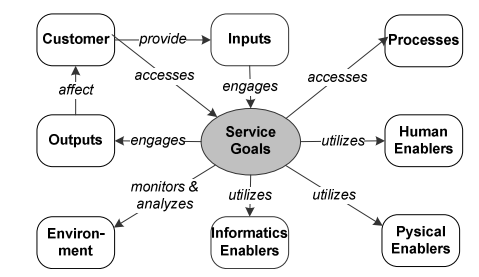
\includegraphics[scale=0.8]{serviceMetaModel}
\caption{Service Meta-Model Entities \cite{Lopes2013}}
\label{fig:MetaModelFig}
\end{center}
\end{figure}\par

The figure \ref{fig:MetaModelFig} above gives easy steps to achieve a service goal. As this research aimed to achieve the same goal, combination of both, service meta model and Hyogo for Action Framework are an opportunity. Developing the smart system to support the disaster mitigation is part of using knowledge, innovation and education to build a culture of  safety and resilience at all levels.\par 
 
The figure \ref{fig:MainPartDM} below, represent main points of disaster management entities. The customer in SDMS should be communities, government and many agencies. The SDMS will receive various inputs from these customers with varying access. The inputs such as customer demands, mental and physic injuries and public safety. We defined customer demand as people or community need when disaster happen. The main need was defined from people area fast warning (early warning) and safe location for evacuation. The government also need to prepare any mental or physical damage at disaster victims. \par 

All customer providing mentioned at paragraph above will be define in the system. From these inputs and customer attributes, SDMS will create the service value chain that will make linkage between secondary part of SDMS. The value of service defined as output from the system. The outputs are customer demand fulfilled, safe customer (people), optimum disaster management and reconstructions and rehabilitations process working fast.\par

\begin{figure}[H]
\begin{center}
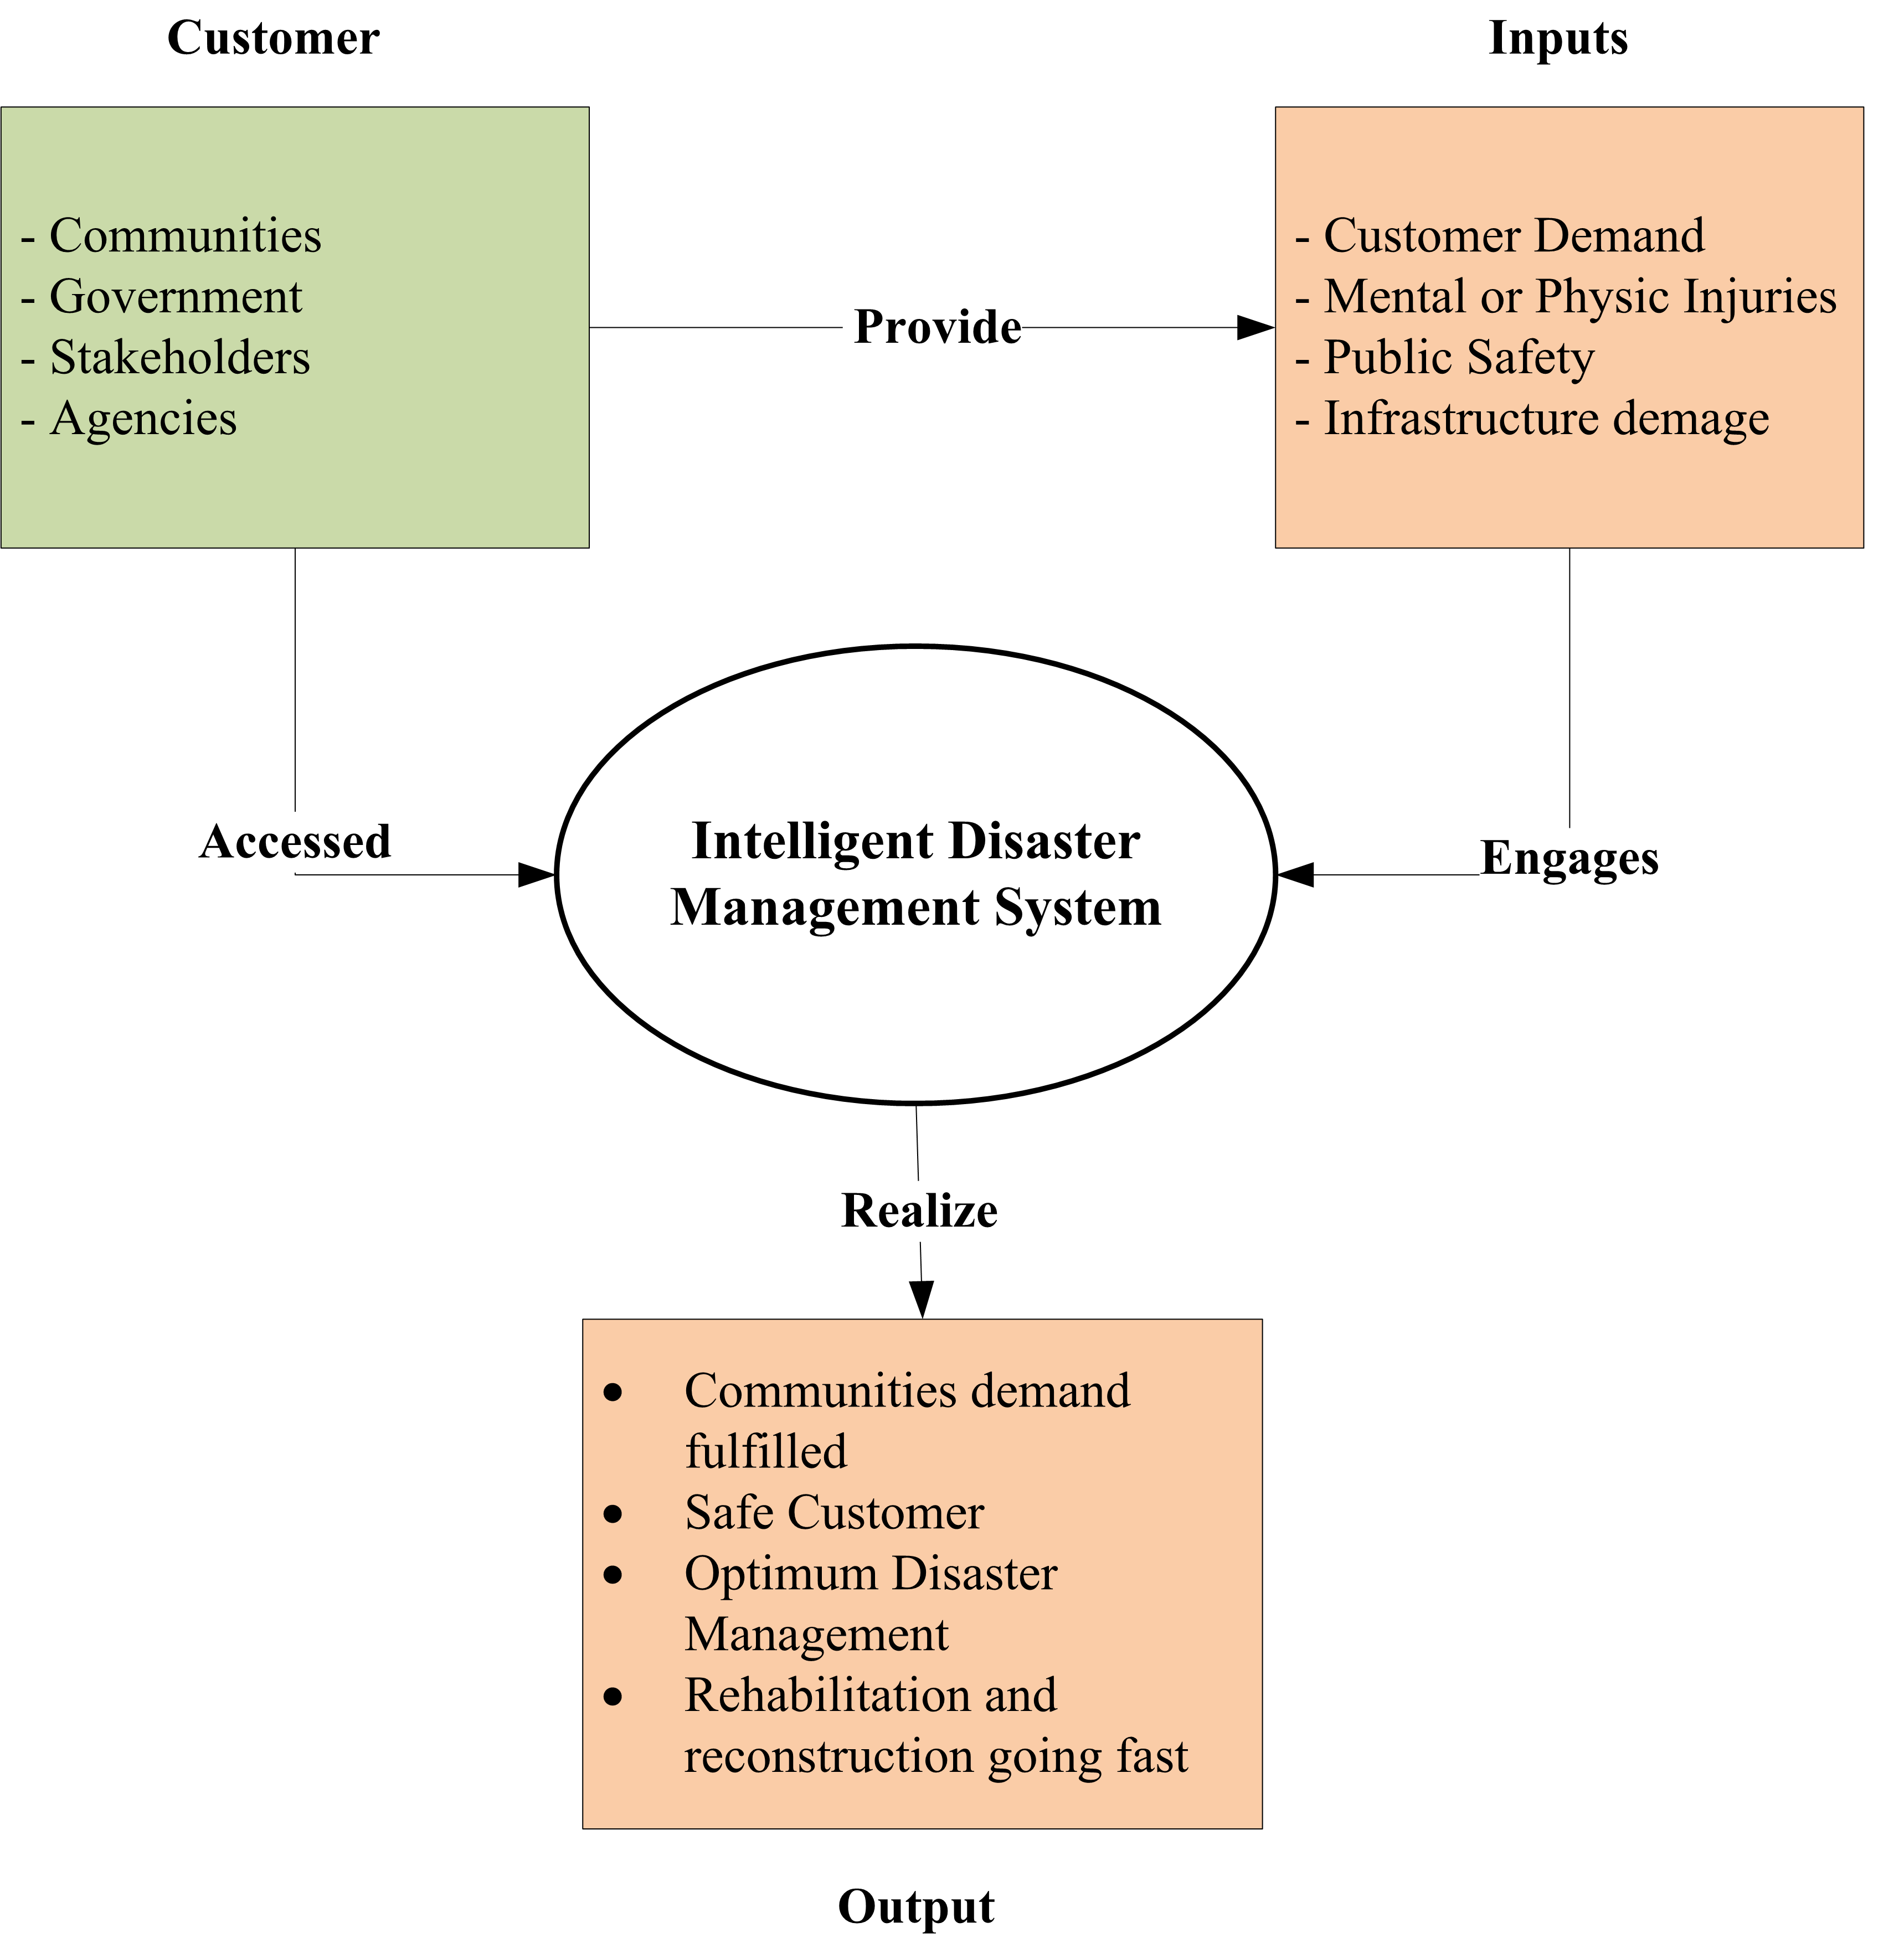
\includegraphics[scale=0.7]{idms.png}
\caption{Main Part of Disaster Management Based on Service}
\label{fig:MainPartDM}
\end{center}
\end{figure}\par

%gambar perlu dijelaskan secara terperinci dan jelas setiap bagian-bagiannya.
The important things of this phase are different communities condition and purposes. people lives in Sumatera island, most of them lives in rural area, and people lives in Java island lives in density area. In consequence, people in Sumatera can mitigate from disaster easier than people in Java. Different approach of area problem  will give solution to identify, asses and monitor disaster risk and enhance early warning system. \par
Secondary part of SDMS are utilizing, executing, monitoring and analyzing. SDMS should be using human enabler, physical enabler and information enablers. Many data from three of them will help SDMS to monitor and analyze environment. Furthermore, executes the processes.\par
 
\subsection{Business Process Identification}
As identification process is an important start to define the form of desired service to be delivered to community. To iterate, the purpose of service innovation is to improve value for communities. Therefore in the identification process there is must be a process to identify potential service of increasing the value, for this process we need a Business Model Canvas (BMC)\cite{SOASImple}. BMC can provide an overview of the Government to identify sector to improve in order to increase the value proposition.\par

\begin{landscape}
\thispagestyle{empty}
\begin{figure}[H]
\centering
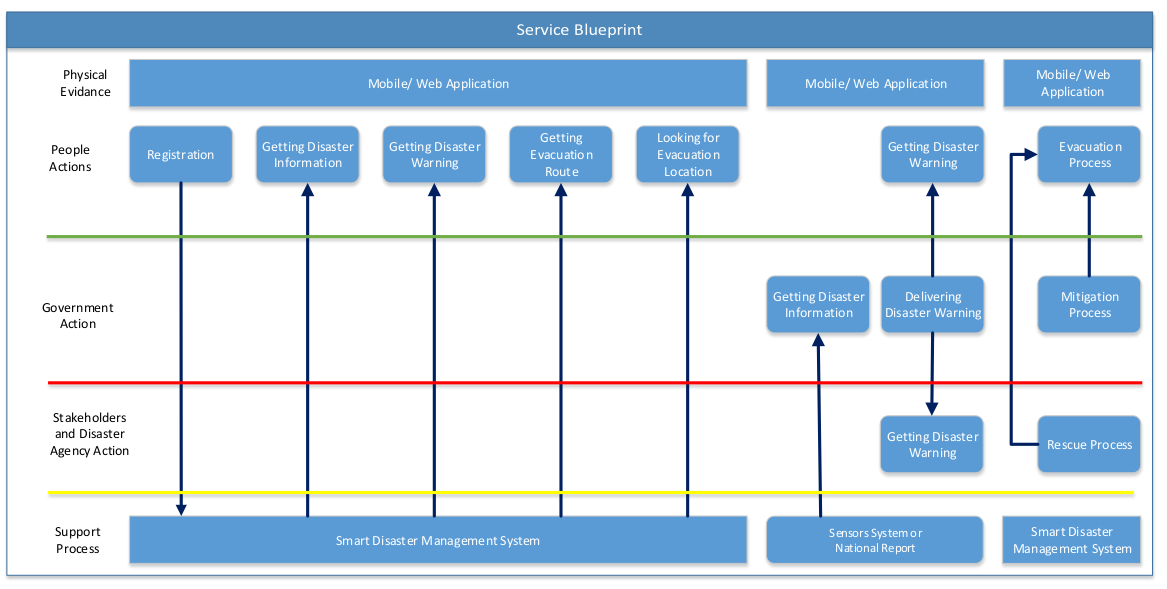
\includegraphics[scale=0.8]{ServiceBlueprint.png}
\caption{Service Blueprint Smart Disaster Management System}
\label{fig:ServiceBlueprint}
\end{figure}
\end{landscape}\par

From the figure \ref{fig:ServiceBlueprint}, there are 3(three) lines to separate the interaction each action,
\begin{enumerate}
\setlength{\itemsep}{1.5pt}
\setlength{\parskip}{1.5pt}
\item Line with yellow color, this shown the interaction of communities as user to the system itself. 
\item Line with red color, the line shown the interaction service of government and stakeholders or disaster agency.
\item Line with green color, the last line shown the interaction between  government and the communities.
\end{enumerate}

The services shown in figure \ref{fig:ServiceBlueprint} are:
\begin{enumerate}
\setlength{\itemsep}{1.5pt}
\setlength{\parskip}{1.5pt}
\item Registration, communities should do this process to help local government saving their information. In this process, user's email address, phone number and their exact location should be inputed. In main condition, internet connectivity may be not work when disaster happen and for that reason, we need another option such as SMS.
\item Getting Disaster Information, People as user will get many disaster informations from mobile application. The informations was given by the government. 
\item Getting Disaster Warning, registered people will directly getting warned by mobile application when disaster happen. 
\item Getting Evacuation Route, the information achieved at registered people not only disaster warning but location of disaster happen. This is important part that evacuation route help people to evacuate precisely and directly without panic.
\item Looking for evacuation Location, this is additional option. People can see the evacuation point around his area. Infrastructure of evacuation point is another main aspect in disaster mitigation to be prepared.
\end{enumerate}

\subsection{Operation Candidates Identification}
In this part, We need to identify the operation candidates from the service blueprint that was designed. According to service blueprint, the operation candidates that possible in the system  are:
\begin{enumerate}
\setlength{\itemsep}{1.5pt}
\setlength{\parskip}{1.5pt}
\item evacuation route information, people can access information of route that will help them evacuate to right location.
\item evacuation location point. User also can access the information of evacuation location.  in future development, we can provide more information such as measure of building, building facilities or amount of evacuee.
\item registration process. Every user have to register their identity and choose different alias. People will register as community, government register as government and stakeholders or other disaster agency have to register as stakeholders. This difference is needed in parting the function in service.
\item Disaster warning notification. Showing the notification to evacuate as soon as possible when this notification coming.
\item Disaster agency information. Showing information of disaster agency or stakeholders that can help the victim in disaster time.
\item Government information. Showing government information, the details to be informed should be determined before.
\item user location. Showing user location information.
\end{enumerate}

\subsection{Logic Abstract Orchestration}
There are logic workflows separated from Both of Operation candidates identification and business process, there are:
\begin{enumerate}
\setlength{\itemsep}{1.5pt}
\setlength{\parskip}{1.5pt}
\item at the first step,user should register to login, if login process is successful user will be directed to main page.
\item if login was failed, user will be directed to choose two button. The first button is register button, and the second one is forgot password button.
\item email with registered user will not be working. 
\item not only email, phone number with registered user also will not be signed up for second time.
\item User can close the application when they finished read the information, and the application still run at back end.
\item User can check his location.
\item User also can ask some information they needed based on current disaster. 
\end{enumerate}

\subsection{Creating Service Candidates}
After getting candidates operation and logic abstract orchestration, the next step is creating service candidates as shown in figure \ref{fig:candidatesService} below:

\begin{figure}[H]
\centering
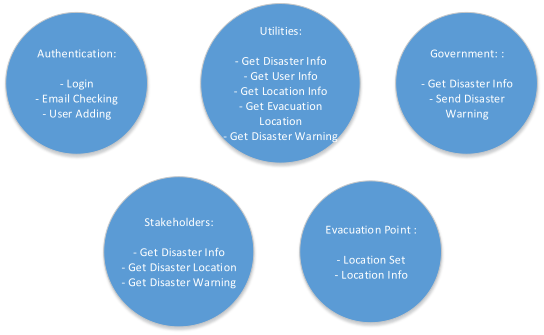
\includegraphics[scale=0.6]{candidatesService.png}
\label{fig:candidatesService}
\caption{Service Candidates}
\end{figure}

\subsection{Service Oriented Implementation and Repairing}
The step is repairing the service candidates that was made, but before jumping to it, a relevant Entity Relation Diagram (ERD) with the system must be defined. The defined ERD is shown in figure \ref{fig:ERDDiagram} below:\par

\begin{figure}[H]
\centering
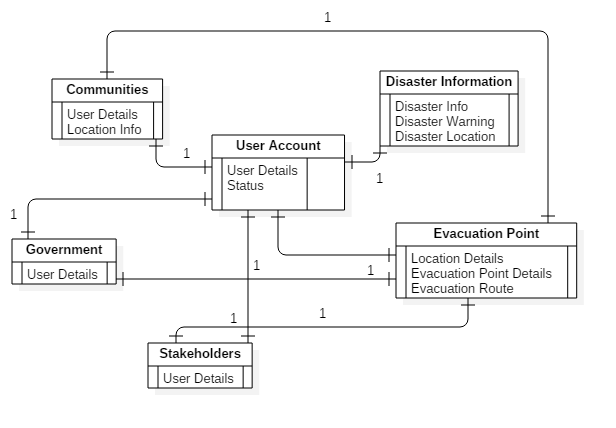
\includegraphics[scale=0.6]{ERDDiagram1.png}
\label{fig:ERDDiagram}
\caption{Entity Relation Diagram}
\end{figure}

The explanation of ERD objects from the figure above are:
\begin{enumerate}
\setlength{\itemsep}{1.5pt}
\setlength{\parskip}{1.5pt}
\item Communities: an object represented people who need to be informed or warned when disaster is happening. In many conditions, user also can access some disaster informations given by government at application.
\item Government, an object represented the user account for government. The government user received disaster information from sensor systems to the application and share it if the information is dangerous and needed to be shared soon.
\item Stakeholders, an object represented as organization user account. The organization is taking a part in helping process after disaster attacking.
\item User Account, an object that represented all user in application. The users include communities, government and stakeholders.
\item Disaster Information, it represented to every information about disaster.
\item Evacuation Point, it represented the locatioan of disaster evacuation that the communities or disaster agency to be when the disaster happen. 
\end{enumerate}\par 

the relations between every entities in figure \ref{fig:ERDDiagram} could be explained in the table \ref{tab: TabelRelationEntity} below:
\begin{table}[h!] 
\begin{center}
\caption{Entity Relation Table}
\label{tab: TabelRelationEntity}
	\vspace{0.1cm}
\begin{tabular}{ |>{\centering\arraybackslash}m{2cm}|>{\centering\arraybackslash}m{3cm}|>{\centering\arraybackslash}m{3cm}|>{\centering\arraybackslash}m{3cm}|>{\centering\arraybackslash}m{3cm}|}
 \hline
 \textbf{Entity} & \textbf{Relation} & \textbf{Min Relation} & \textbf{Max Relation} & \textbf{Entity Name}\\
 \hline \hline
 Communities & accessed & 1 to 1 & 1 to 1 & Disaster Info\\
 \hline 
 Government & accessed & 1 to 1 & 1 to 1 & Disaster Info\\
 \hline
 Stakeholders or Disaster Agency & Accessted & 1 to 1 & 1 to 1 & Disaster Info\\
 \hline
 Evacuation Point & accessed & 1 to 1 & 1 to 1 &  Evacuation Point location\\
 \hline
\end{tabular}
\end{center}
\end{table}\par

After ERD process defined, service candidates can be redefined. Adaptability process is for completing service candidates identification process. service candidates that being adaptable is shown in figure below:

\begin{enumerate}
\setlength{\itemsep}{1.5pt}
\setlength{\parskip}{1.5pt}
\item Adding notification service as service candidate. 
\item Adding Disaster Info service as service candidate.
\item Adding detais informations from each type of user account.
\end{enumerate}

%% gabar perlu disesuaikan kembali
\begin{figure}[H]
\centering
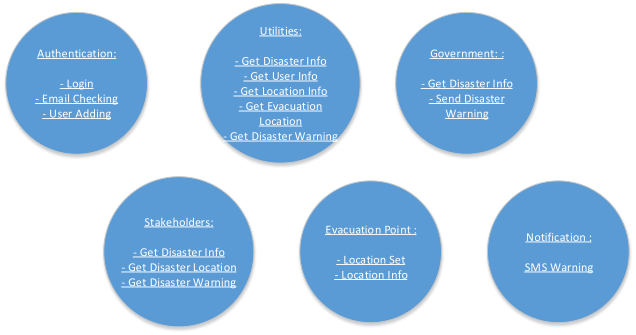
\includegraphics[scale=0.7]{reidentifiedService.png}
\label{fig:ReServiceComposition}
\caption{Service Composition re-identified}
\end{figure}

\subsection{Service Composition Identification}
This step is to identify service candidates that have been made
previous to put in the orchestration layer, the business layer, or
the application layer. Figure \ref{fig:ServiceComposition} illustrates the composition identification service.

\begin{figure}[H]
\centering
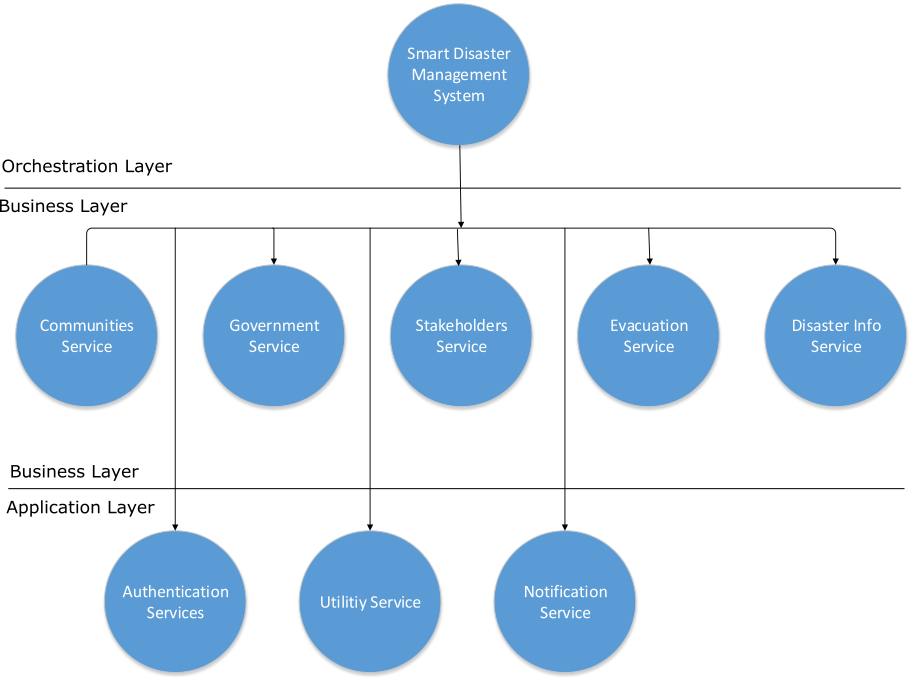
\includegraphics[scale=0.6]{ServiceComposition.png}
\label{fig:ServiceComposition}
\caption{Service Composition}
\end{figure}

\subsection{Reviewing The Operation Candidates}
This step is reviewing the composition of the service that has been previously identified, Smart Disaster Management System, there are several services
which should be adjusted to be grouped into other services, including:

\subsection{Processing Analysis Needed}
SDMS business process is not complex, and it has identified all
candidate preparation service that illustrates the logic of the application. Therefore,
This step is not required in the SDMS.

\subsection{Application Service Operation Identification}
This step describe the process of service operation in the application, which is 
illustrated by the sequence diagram in figure :

\begin{enumerate}
\setlength{\itemsep}{1.5pt}
\setlength{\parskip}{1.5pt}
\item Sequence Diagram of authentication service
\begin{figure}[H]
\centering
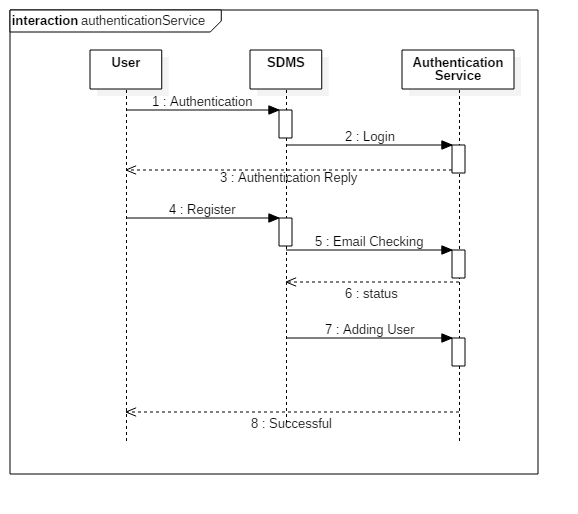
\includegraphics[scale=0.5]{authenticationService.png}
\label{fig:AutService}
\caption{Authentication Service}
\end{figure}

\item Sequence diagram of utility services
\begin{figure}[H]
\centering
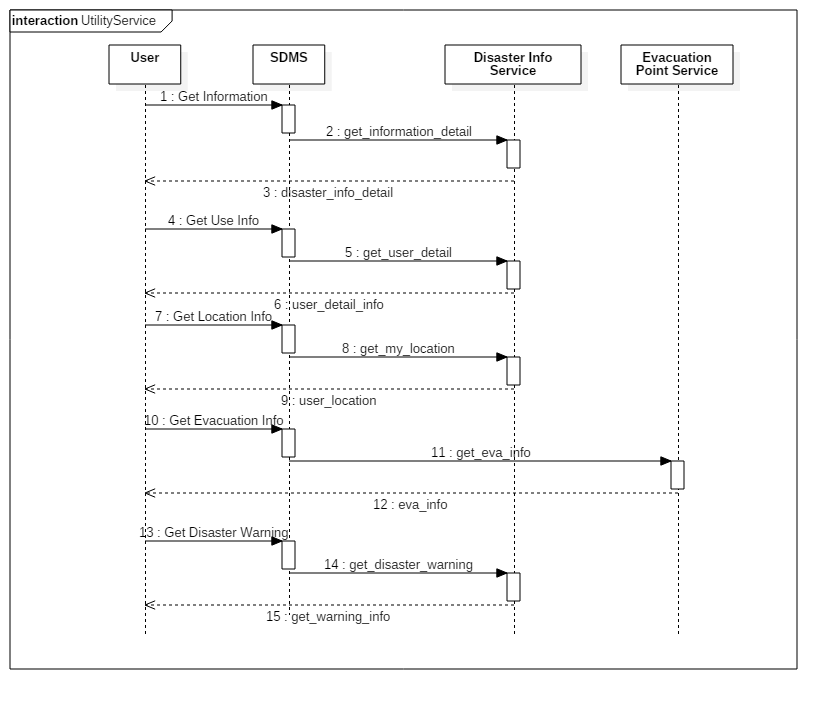
\includegraphics[scale=0.4]{UtilityService.png}
\label{fig:UtiService}
\caption{Utility Services}
\end{figure}

\item Sequuence diagram of government service
\begin{figure}[H]
\centering
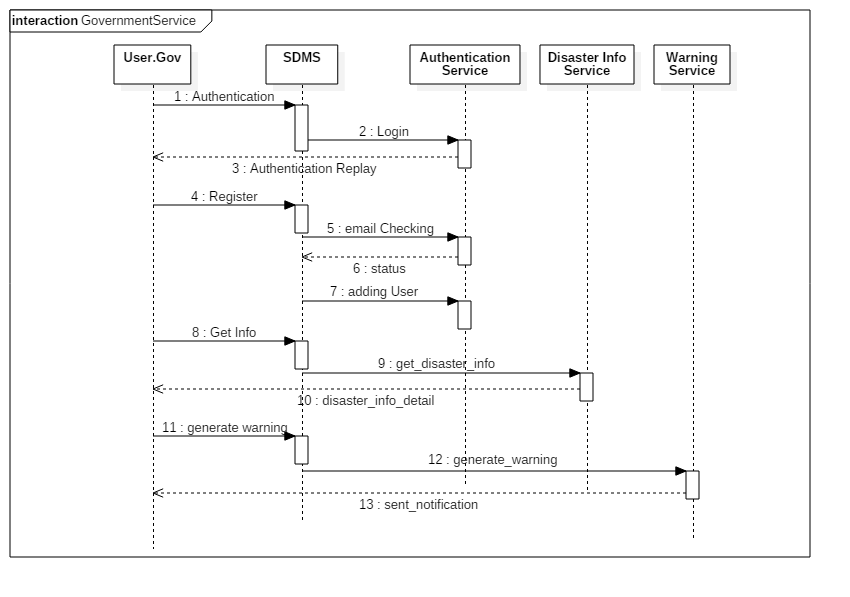
\includegraphics[scale=0.4]{GovernmentService.png}
\label{fig:GovService}
\caption{Government Service Diagram}
\end{figure}

\item Sequuence diagram of stakeholder service
\begin{figure}[H]
\centering
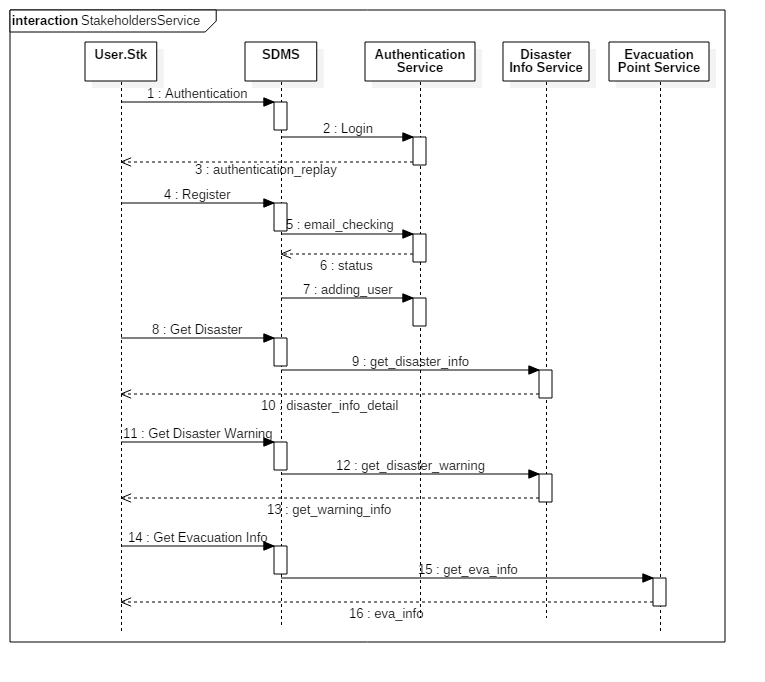
\includegraphics[scale=0.5]{StakeholdersService.png}
\label{fig:StkService}
\caption{Stakeholder and Disaster Agency Service}
\end{figure}

\item Sequuence diagram of evacuation point service
\begin{figure}[H]
\centering
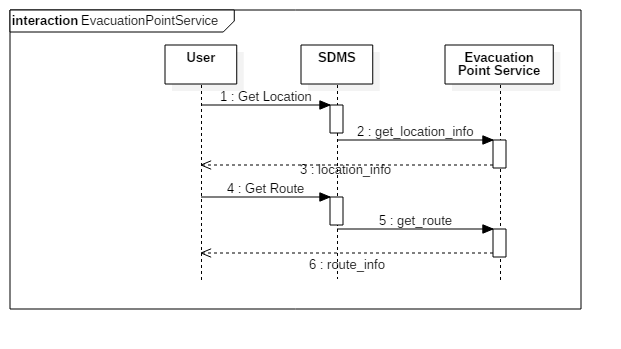
\includegraphics[scale=0.5]{EvacuationPointService.png}
\label{fig:EvaPointService}
\caption{Evacuation Point Service}
\end{figure}
\end{enumerate}

\subsection{Creating Application Service Candidates}
Identifications and specifications service design is needed to be changed to technical services, or usually known as application services or web services. The table 

\begin{table}[h!]
\begin{center}
\normalsize
\caption{Application Service Candidates}
\label{tab: AppServCand}
	\vspace{0.1cm}
\begin{tabular}{ |>{\centering\arraybackslash}m{1cm}|>{\centering\arraybackslash}m{3cm}|>{\centering\arraybackslash}m{5cm}|>{\centering\arraybackslash}m{3cm}|}
 \hline
 \textbf{No.} & \textbf{Application Service} & \textbf{Output} & \textbf{Parameters}\\
 \hline \hline
 1. & Login & success: boolean & username: string, password: string\\
 \hline 
 2. & CheckEmail & success: boolean & email: string \\
 \hline
 3. & AddUser & success: boolean & list $<$User Attribute$>$ \\
 \hline
 4. & GetDisInfo & List $<$DisInfoAttribute$>$ & code: string\\
 \hline
 5. & GetLocation & List $<$LocationAttribute$>$ & longitude: double, latitude: double \\
 \hline
 6. & GetEvaPointInfo & List $<$EvaPointAttribute$>$ & longitude: double, latitude: double  \\
  \hline
 7. & GetRoute & List $<$RouteAttribute$>$ & longitude: double, latitude: double  \\
  \hline
 8. & GetDisWarn & List $<$WarnAttribute$>$ & code: string \\
 \hline
 %%9. & GetDisInfo & 1 to 1 & 1 to 1 \\
 %%\hline
 %%10. & GetDisInfo & 1 to 1 & 1 to 1 \\
 %%\hline
\end{tabular}
\end{center}
\end{table}\par

%%\begin{comment}
%%\end{comment}


\subsection{Reviewing Service Compositions}
This step is the reviewing process of service compositions that was designed before. actually, for smart disaster management system, the compositions service was defined before and in consequence does not need to be reviewed.

\subsection{Reviewing Operation Candidates}
This step is also defined before, in consequence this step can be skipped to the next step.
\section{Service Oriented Designing}
\vspace{-0.5cm}
\subsection{Composing SOA}
As mentioned in this research, SOA in an element to develop the smart disasteranagement system. There 3(three) parts in composing SOA, selecting service ayerdefining the core standard and the last is selecting SOA extension. Each part of them wil be explained below.

\subsubsection{Service Layer Selecting}
There are 3(three) layers to be used in this SOA composing. Orchestration layer, business layer and application layer. All of them have been explained before in figure \ref{fig:ServiceComposition}.

\subsubsection{Core Standards Position}
This step is core standard designing step. The design will be used in web service. The figure below is shown the core standard used in smart disaster management system.

\subsubsection{SOA Extension Selecting}
SOA extension that will be used in SOA composing is WS-sdms.

\section{Application Designing}
The prototype will be build to support the system. The prototype is going to build in mobile application and web application that used every services explained before. This explanation focused at architecture function and design function fro the system built. The development will follow the business process step and SOA design that defined before.\par  
Designing of structure and function will be defined by use case diagram, and user interface will created for mobile application and web application. There areany ways to create the application, but in this research the easiest part will be used. Application will be built using HTML 5. In addition as easy programming, HTML 5 is also based on web application, so it will help us when the application needs the maintenance. The compatibly of HTML 5 with many devices is also a reason in creating this application.The compatibly of HTML 5 is shown at figure \ref{fig:html5}. \par 

\begin{figure}[H]
\centering
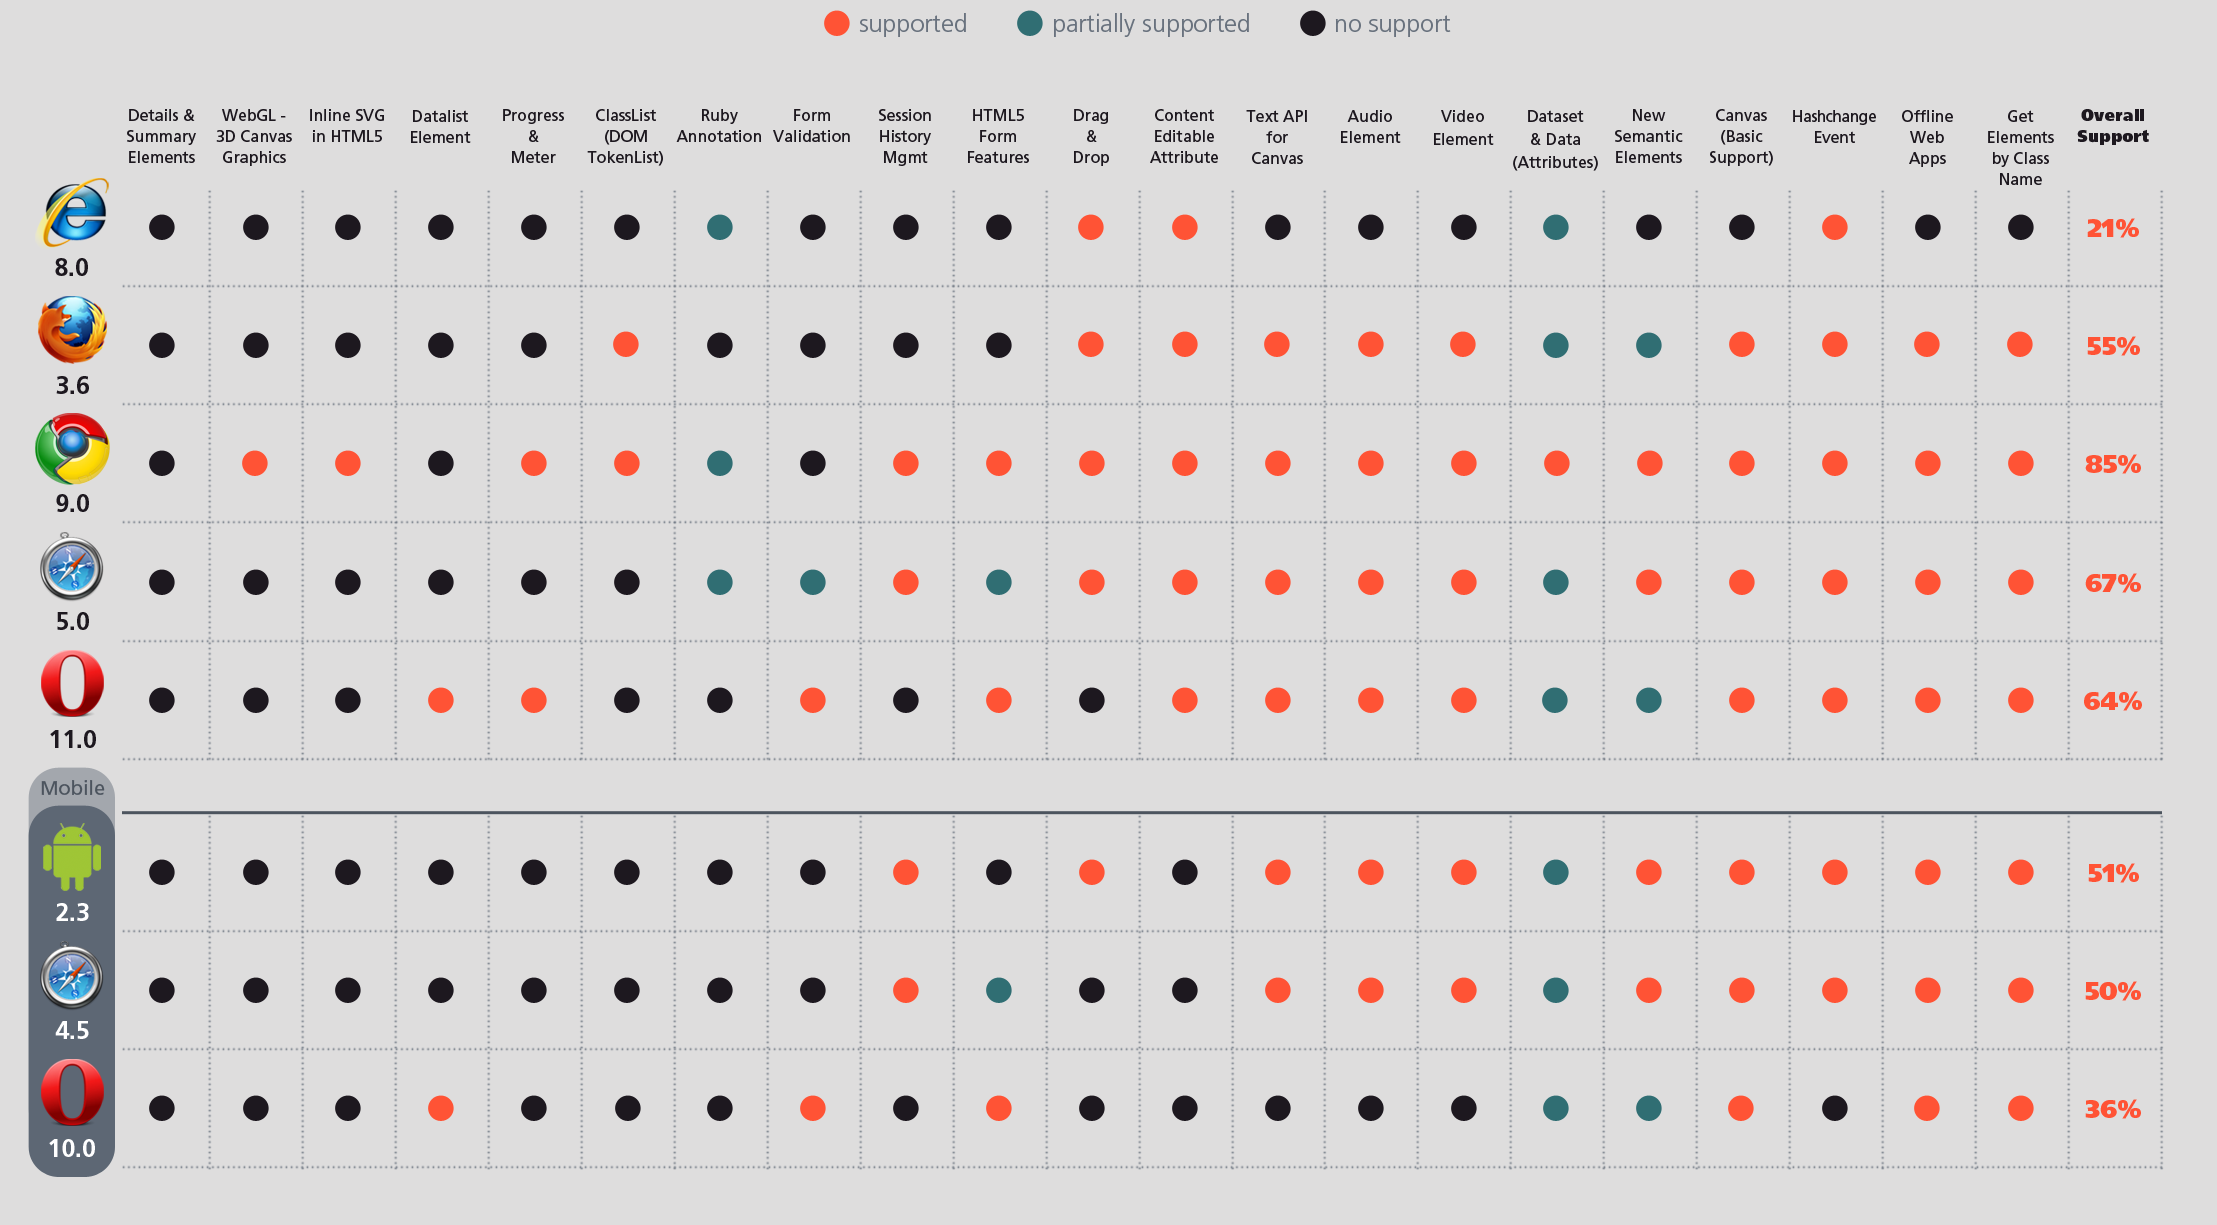
\includegraphics[scale=0.25]{html5.png}
\label{fig:html5}
\caption{The Compatibly of HTML 5 with Web Applications \cite{HTML5}}
\end{figure}

\section{Use Case Diagram}
Use case diagram are determined on basic functions needed. Basic functions are defined in use case diagram is helping to make the application easier to understand and all needed will be accommodated in use case diagram. A next explanations will cover the explanations of use case diagram was defined.

\begin{enumerate}
\item User (Communities)\par 
community user account is main actor in this system. The community start using the application by login to it. After login, user can access disaster information, evacuation point information and getting warning notification.  
\begin{figure}[H]
\centering
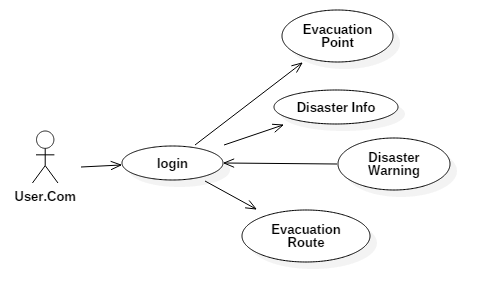
\includegraphics[scale=0.4]{UserComDiagram.png}
\label{fig:comUseCase}
\caption{Community Use Case Diagram}
\end{figure}

The explanation of use case  diagram above is:
\begin{table}[H]
\begin{center}
\caption{Community Use Cases Diagram}
\label{tab: ComUCDiagram}
	\vspace{0.1cm}
\begin{tabular}{ |>{\centering\arraybackslash}m{2cm}|>{\centering\arraybackslash}m{4cm}|>{\centering\arraybackslash}m{6.5cm}|}
 \hline
 \textbf{Actors} & \textbf{Use Cases} & \textbf{Descriptions} \\
 \hline \hline
  (AK01) User Community & (UC01) Disaster Info & This function used for getting disaster information which that provided from government or from sensor system directly. \\
 \hline 
 & (UC02) Evacuation Point & This function used for searching the location of evacuation points. In some condition, evacuation points is depend on the government. \\
 \hline
 & (UC03) Disaster Warning & This function used for getting warning of disaster happen. Its also a warning to do evacuation process to user received the warning. \\
 \hline 
 & (UC04) Disaster Route This function used for user get best way to run when they get the warning to evacuate& \\
 \hline
 %%\hline
\end{tabular}
\end{center}
\end{table}

\item User (Government)\par
Government is has another initial user account. When register process, they will directed to choose as government. As the government, user will get disaster information and sent warning notification to both other user account (Community and Stakeholder).

\begin{figure}[H]
\centering
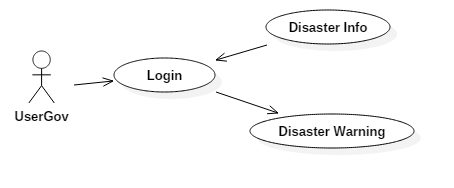
\includegraphics[scale=0.4]{UserGovDiagram.png}
\label{fig:govUseCase}
\caption{Government Use Case Diagram}
\end{figure}

The explanation of use case  diagram above is:
\begin{table}[H]
\begin{center}
\caption{Community Use Cases Diagram}
\label{tab: ComUCDiagram}
	\vspace{0.1cm}
\begin{tabular}{ |>{\centering\arraybackslash}m{2cm}|>{\centering\arraybackslash}m{4cm}|>{\centering\arraybackslash}m{6.5cm}|}
 \hline
 \textbf{Actors} & \textbf{Use Cases} & \textbf{Descriptions} \\
 \hline \hline
  (AK02) User Government & (UC05) Disaster Info & This function used for getting disaster information which that provided from government or from sensor system directly. \\
 \hline 
 & (UC06) Disaster Warning & This function used for sending the warning message to other two both user, community and stakeholders. \\
 \hline 
 %%\hline
\end{tabular}
\end{center}
\end{table}

\item User (Stakeholder)\par 
Stakeholder account actually same like community account. The difference between two of them is at limited service they get. Stakeholders account only get warning notification and evacuation point. Both are important in stakeholder.
\begin{figure}[H]
\centering
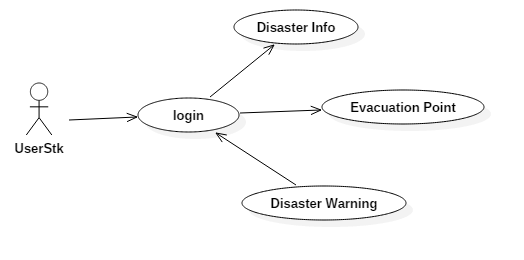
\includegraphics[scale=0.4]{UserStkDiagram.png}
\label{fig:stkUseCase}
\caption{Stakeholder Use Case Diagram}
\end{figure}

The explanation of use case  diagram above is:
\begin{table}[H]
\begin{center}
\caption{Stakeholders Use Cases Diagram}
\label{tab: stkUCDiagram}
	\vspace{0.1cm}
\begin{tabular}{ |>{\centering\arraybackslash}m{2cm}|>{\centering\arraybackslash}m{4cm}|>{\centering\arraybackslash}m{6.5cm}|}
 \hline
 \textbf{Actors} & \textbf{Use Cases} & \textbf{Descriptions} \\
 \hline \hline
  (AK03) User Stakeholders & (UC07) Disaster Info & This function used for getting disaster information which that provided from government or from sensor system directly. \\
 \hline 
 & (UC08) Evacuation Point & This function used for searching the location of evacuation points. In some condition, evacuation points is depend on the government. \\
 \hline
 & (UC09) Disaster Warning & This function used for getting warning of disaster happen. Its also a warning to do evacuation process to user received the warning. \\
 \hline 
 %%\hline
\end{tabular}
\end{center}
\end{table}
\end{enumerate}

All use cases are mentioned can be explained in one figure as shown as figure \ref{fig:MainUseCase}:
\begin{figure}[H]
\centering
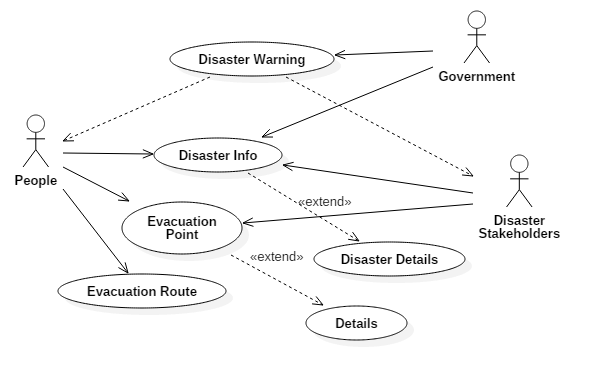
\includegraphics[scale=0.5]{MainUseCaseDiagram.png}
\label{fig:MainUseCase}
\caption{Complete Use Cases Diagram of the System}
\end{figure}

\section{Technology Architecture}
This section will explain about technology used in service implementing process. There are different technology was used in developing, and which difference used was based on needed from the system.
\begin{enumerate}
\item Web base application. Using Service Oriented Architecture made the application need a web application in implementation. Its because between user interface at application can not be separated with the service available.
\item Short Message Service (SMS), event internet is the main technology today, we need a back up technology to support the application in rural area. Rural area is not only a reason for implementing the SMS, many people in local area still using SMS in main way of communicating each other.
\item Cloud Computing Technology. The familiar technology is used now days. Easy access in many ways for user. This technology help user to access the application with his smart phone, tablet, laptop or computer device. 
\end{enumerate}
The explanation above can be defining in figure \ref{fig:TechUsed}:
\begin{figure}[H]
\centering
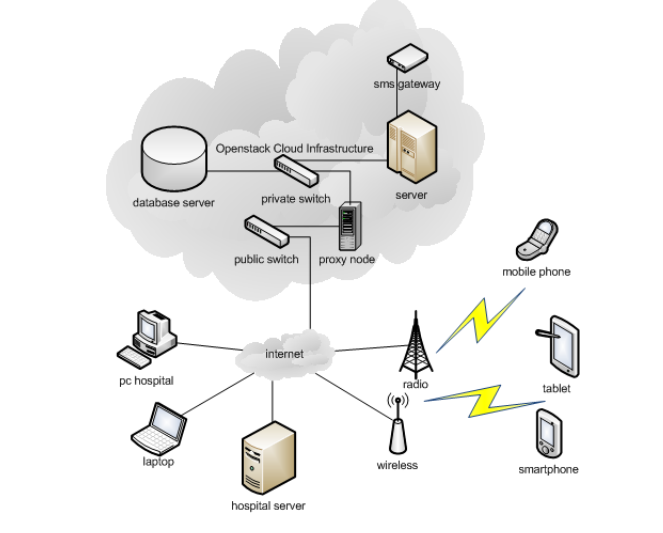
\includegraphics[scale=0.6]{techUsed.png}
\label{fig:TechUsed}
\caption{Technology Architecture Used in Smart Disaster Management System}
\end{figure}


\begin{comment}
\begin{table}[h!]
\begin{center}
\caption{Application Service Candidates}
\label{tab: AppServCand}
	\vspace{0.1cm}
\begin{tabular}{ |>{\centering\arraybackslash}m{2cm}|>{\centering\arraybackslash}m{3cm}|>{\centering\arraybackslash}m{5cm}|}
 \hline
 \textbf{Actors} & \textbf{Use Cases} & \textbf{Descriptions} \\
 \hline \hline
  &  &  \\
 \hline 
 &  &  \\
 \hline
 &  &  \\
 \hline
 &  & \\
 \hline
 %%\hline
\end{tabular}
\end{center}
\end{table}\par
\end{comment}